\documentclass[12pt]{report}
\usepackage[a4paper]{geometry}
\usepackage[myheadings]{fullpage}
\usepackage{fancyhdr}
\usepackage{lastpage}
\usepackage{graphicx, wrapfig, subcaption, setspace, booktabs}
\usepackage[T1]{fontenc}
\usepackage[font=small, labelfont=bf]{caption}
\usepackage{fourier}
\usepackage[protrusion=true, expansion=true]{microtype}
\usepackage[german]{babel}
\usepackage{sectsty}
\usepackage{url, lipsum}

\makeatletter
\patchcmd{\chapter}{\if@openright\cleardoublepage\else\clearpage\fi}{}{}{}
\makeatother

\newcommand{\HRule}[1]{\rule{\linewidth}{#1}}
\onehalfspacing
\setcounter{tocdepth}{5}
\setcounter{secnumdepth}{5}

%-------------------------------------------------------------------------------
% HEADER & FOOTER
%-------------------------------------------------------------------------------
\pagestyle{fancy}
\fancyhf{}
\setlength\headheight{15pt}
\fancyhead[L]{Haller Tobias}
\fancyhead[R]{HTBLuVA Wiener Neustadt}
\fancyfoot[R]{Page \thepage\ of \pageref{LastPage}}
%-------------------------------------------------------------------------------
% TITLE PAGE
%-------------------------------------------------------------------------------

\begin{document}

\title{ \normalsize
		\\ [2.0cm]
		\HRule{0.5pt} \\
		\LARGE \textbf{\uppercase{Aufgabe 4.1 \\ Digest basierte Authentifizierung}}
		\HRule{2pt} \\ [0.5cm]
		\normalsize \today \vspace*{5\baselineskip}}

\date{März 2023}

\author{
        Haller Tobias, 5AHIF \\
		Katalognummer: 4 \\ 
		HTBLuVA Wiener Neustadt \\
        Abteilung Informatik }

\maketitle
\tableofcontents
\newpage

%-------------------------------------------------------------------------------
% Section title formatting
\sectionfont{\scshape}
%-------------------------------------------------------------------------------

%-------------------------------------------------------------------------------
% BODY
%-------------------------------------------------------------------------------

\chapter{Aufgabenstellung}
Simulation einer Digest-baiserte Authentifizierung auf einer Website. Dabei werden ein Client und ein Server simuliert, auf der Client-Seite werden die Anmeldedaten per Konsole oder über eine Config-Datei eingelesen. Nach dem Authentifizierungsprozess beendet sich der Client und der Server ist für eine neue Anfrage bereit.

\chapter{Digest-basierte Authentifikation - Theorie}
\subsection{Allgemeines}
Digest-basierte Authentifizierung ist ein Weg für Service-Provider eine Person aufgrund ihrer Anmeldeinformation mit der Benutzung eines Webbrowser zu verifzieren. Digest-basierte Authentifizierung benutzt das HTTP-Protkoll und verwendet MD5-Hashing, sowie eine Nonce (einmalig generierte Zeichenfolge) um wiederholende Attacken abzuwehren. Die generierten Hashes werden an den Benutzernamen und das Kennwort der Person angehängt, bevor sie über das Netzwerk gesendet werden, so dass der Server des Providers die Person authentifizieren kann. Diese Art der Authentifizierung wird der klassichen Basic-HTTP-Authentifizierung vorgezogen, da es unsicheres Base64-Encoding verwendet. 

\subsection{Vorteile/Nachteile der Digest-basierten Authentifikation}
Die Vorteile dieser Arten der Authentifikation sind:
\begin{itemize}
    \item Das Passwort wird nicht klar an den Server gesendet. 
    \item Das Passwort ist nicht direkt gehasht sondern in Kombination mit Username, Realm. 
    \item Die Client-Nonce erlaubt, das Verhindern von \textit{Chosen-Plaintext-Attacken}, sowie \textit{Rainbow-Table-Attacken}. 
    \item Die Server-Nonce erlaubt Zeitstempel um wiederholende Attacken zu verhindern. Der Server ist auch erlaubt eine Liste von bereits genutzen Noncen zu speichern 
    \item \textit{Phishing-Attacken} werden durch das Hashing des Passworts verhindert. 
\end{itemize}
Die Nachteile sind:
\begin{itemize}
    \item Die Webseite hat keine Kontrolle über das UI, welches den End-Benutzer gezeigt wird.
    \item Viele der Sicherheitsoptionen sind optional.
    \item Digest-basierte Authentifikation ist für eine \textit{man-in-the-middle-Attacke} anfällig. 
    \item Der Server speichert den HA1-Hash, welcher das Passwort beinhaltet. Damit kann er sich dann bei einem Datenleak trotz Verschlüsselung authentifizieren. 
    \item Die Verwendung von starken Passwörtern wird verhindert, da entweder Passwort, Username oder Realm und Passwort wiederherstellbar sein müssen. 
\end{itemize}

\chapter{Implementierung}
\begin{figure}[h]
 \centering
 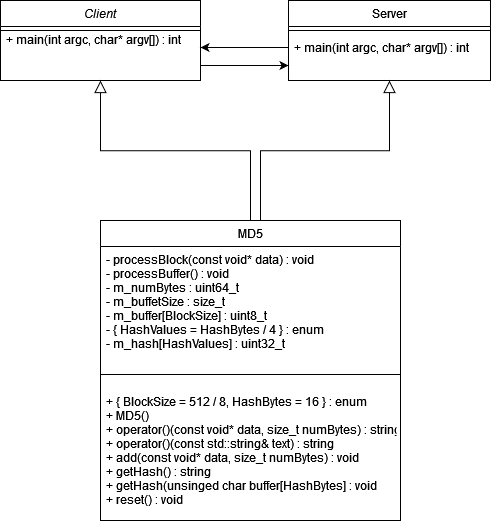
\includegraphics[width=10cm,height=10cm]{DigestBasierteAuthUML.png}
 \caption{Übersichtdiagramm Digest-basierte Authentifizierung}
 \label{fig:Profil}
\end{figure}

Bei den Code Beispielen werden diese Namespaces verwendet.
\begin{verbatim}
using namespace std;
using namespace asio::ip;
\end{verbatim}

\subsection{Ablauf der Authentifizierung}
\begin{enumerate}
    \item Zuerst sendet der Client einen String mit ''LOGON'' und einer Digest-URI an den Server.
    \item Der Server liest diese Anfrage und prüft durch ''LOGON'' ob es sich um eine Authentifizierungsanfrage handelt. Der Server prüft dannach ob die angegebene URI auch für eine Verifizierung geeignet ist. 
    \item Der Server sendet den Client dann den zugehören Realm zur URI und eine zufällig berechnete Nonce.
    \begin{verbatim}
unsigned int generateNonce() {
    random_device rd; 
    mt19937 gen(rd()); 
    uniform_int_distribution<unsigned int> distrib(0, UINT_MAX);
    return distrib(gen);
}
    \end{verbatim}
    \item Der Client liest den Realm und die Nonce und generiert sich mithilfe dieser Informationen und den Credentials des Users die Hashes, den ''Reponse''-Hash, welcher dann gesendet wird. (MD5 wird von einer externen Libary bereitgestellt)
    \begin{verbatim}
string generateHashes(string username, string password, string uri, 
                      string realm, unsigned int nonce) {
    string ha1 = username + realm + password;
    string ha2 = "GET" + uri;
    MD5 md5;
    string responseCalc = md5(md5(ha1)+to_string(nonce)+md5(ha2));
    return responseCalc;
}
    \end{verbatim}    
    \item Der Server liest den Response und berechnet auch den gleichen Hash, diese beiden Werte werden dann verglichen und wenn sie gleich sind sendet der Server den Client ein ''ACK'' mit der Nonce. Wenn nicht gleich wird ein ''NAK'' gesendet. 
    \item Der Client liest die Antwort vom Server, gibt sie auf der Konsole aus und beendet sich.
\end{enumerate}

\subsection{Ablauf der Verbindung des Clients mit dem Server}
Zur Verbindung des Clients mit dem Server wird die C++ Libary asio benutzt. Es ist eine Bibliothek zur Netzwerkprogrammierung.
\begin{enumerate}
    \item Zuerst legt der Server einen IO-Stream an mit dem sich der Server verbinden kann.
    \begin{verbatim}
asio::io_context ctx;
tcp::endpoint ep{tcp::v4(), port};
tcp::acceptor acceptor{ctx, ep}; 
acceptor.listen();
tcp::socket sock{ctx};
    \end{verbatim}
    \item Danach verbindet sich der Client auf den Server.
    \begin{verbatim}
tcp::iostream stream("localhost", to_string(port));
    \end{verbatim}
    \item Der Server nimmt die Anfrage an. Durch die while-Schleife, beenden sich der Server nach Abarbeitung der Anfrage nicht und ist für weitere Anfragen bereit.
    \begin{verbatim}
while(true) {
    acceptor.accept(sock);
    tcp::iostream strm{move(sock)
};
    \end{verbatim}
\end{enumerate}
\newpage
\chapter{Quellen}
\begin{itemize}
    \item Digest-basierte Authentifizierung Theorie 
    \url{https://en.wikipedia.org/wiki/Digest\_access\_authentication}
    \item Externer Hashing-Libary 
    \url{https://github.com/stbrumme/hash-library/blob/master/md5.cpp}
\end{itemize}

\end{document}